
\chapter{Kasthreyfing}

\begin{quote}
    \textit{\duck{It's not the fall that kills you; it's the sudden stop at the end.}}
    \begin{flushright}
    - Douglas Adams
    \end{flushright}
\end{quote}

Staða, hraði og hröðun eru vigrar. Hingað til höfum við hunsað það og aðeins skoðað gangfræði í einni vídd. Nú skulum við skoða hvað gerist ef að við látum stöðuna okkar vera vigur í tveim víddum (það er síðan einfalt að sjá hvernig við alhæfum upp í þrjár víddir eftir að við höfum kynnst tveim víddum). Þá getum við ritað:
\begin{align*}
\vec{s} = \begin{pmatrix}
x \\
y
\end{pmatrix}
\end{align*}
Hér tákna $x,y$ lárétta og lóðrétta staðsetningu hlutarins. Hraðinn verður síðan
\begin{align*}
\vec{v} = \frac{d\vec{s}}{dt} = \begin{pmatrix}
v_x \\
v_y
\end{pmatrix}, \hspace{0.5cm} \text{og hröðunin verður} \hspace{0.5cm} \vec{a} = \frac{d\vec{v}}{dt} = \begin{pmatrix}
a_x \\
a_y
\end{pmatrix}.
\end{align*}
Hér táknar $v_x$ hraði hlutarins í lárétta stefnu, $v_y$ hraða hlutarins í lóðrétta stefnu, $a_x$ táknar hröðun hlutarins í lárétta stefnu og $a_y$ táknar hröðun hlutarins í lóðrétta stefnu. Jöfnurnar sem við höfðum leitt út fyrir gangfræði í einni vídd verða allar nákvæmlega eins nema nú á vigra formi. Við höfum þá stöðujöfnurnar:

\begin{tcolorbox}
\begin{theorem}
Lítum á hlut sem er upphaflega staddur í $\vec{s}_0$ og hefur upphafshraða $\vec{v}_0$. Gerum ráð fyrir að hluturinn verði fyrir fastri hröðun $\vec{a}$. Látum $\vec{s}$ tákna stöðu hlutarins og $\vec{v}$ tákna hraða hlutarins eftir tímann $t$. Þá gilda stöðujöfnurnar:

\begin{enumerate}[label = \textbf{(\roman*)}]
    \item $\vec{v} = \vec{v}_0 + \vec{a}t$.

    \item $\vec{s} = \vec{s}_0 + \vec{v}_0 t + \frac{1}{2}\vec{a}t^2$.
    
    \item $2\vec{a} \vdot (\vec{s} - \vec{s}_0) = v^2 - v_0^2$.
\end{enumerate}
\end{theorem}
\end{tcolorbox}

Ef við prófum að skrifa út hvað þessar jöfnur eru að segja þá höfum við að stöðujöfnurnar gilda hnit fyrir hnit, þ.e.a.s.

\begin{align*}
    \vec{v} = \vec{v}_0 + \vec{a}t \hspace{0.5cm} \text{er það sama og} \hspace{0.5cm} \begin{pmatrix}
v_{x}\\
v_{y} \\
\end{pmatrix} = \begin{pmatrix}
v_{x,0}\\
v_{y,0} \\
\end{pmatrix} + \begin{pmatrix}
a_x\\
a_y \\
\end{pmatrix} t = \begin{pmatrix}
v_{x,0} + a_x t\\
v_{y,0} + a_y t \\
\end{pmatrix}
\end{align*}

\begin{align*}
    \vec{s} = \vec{s}_0 + \vec{v}_0 t + \frac{1}{2}\vec{a}t^2 \hspace{0.5cm} \text{er það sama og} \hspace{0.5cm} \begin{pmatrix}
x\\
y \\
\end{pmatrix} = \begin{pmatrix}
x_0\\
y_0 \\
\end{pmatrix} + \begin{pmatrix}
v_{x,0}\\
v_{y,0} \\
\end{pmatrix} t + \frac{1}{2} \begin{pmatrix}
a_x\\
a_y \\
\end{pmatrix} t^2 = \begin{pmatrix}
x_0 + v_{x,0} + \frac{1}{2}a_x t^2\\[2pt]
y_0 + v_{y,0} + \frac{1}{2}a_y t^2
\end{pmatrix}
\end{align*}
\begin{align*}
       2\vec{a} \vdot (\vec{s} - \vec{s}_0) = v^2 - v_0^2 \hspace{0.5cm} \text{er það sama og} \hspace{0.5cm} 2\left( a_x (x-x_0) + a_y (y - y_0) \right) = \left( {v_x}^2 + {v_y}^2 \right) - \left( {v_{x,0}}^2 + {v_{y,0}}^2 \right).
\end{align*}
Þannig í stað þess að vera með þrjár stöðujöfnur þá höfum við tæknilega séð fimm núna.

\section{Að kasta bolta yfir horni}

Hugsum okkur nú að við köstum bolta með upphafshraða $\vec{v}_0$ yfir horni $\theta$ miðað við lárétt (sjá mynd \ref{fig:kasta} hér fyrir neðan). Við viljum skilja hreyfilýsingu boltans eftir að hann yfirgefur hönd þess sem kastar.

\begin{figure}[H]
    \centering
    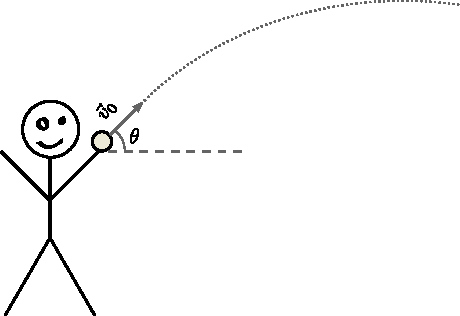
\includegraphics{figures/kasta2.pdf}
    \caption{Matti kastar bolta með upphafshraða $\vec{v}_0$ yfir horni $\theta$ miðað við lárétt.}
    \label{fig:kasta}
\end{figure}
Það er þess vegna sniðugt að brjóta upp upphafshraða boltans í lárétta og lóðrétta stefnu, við höfum að:
\begin{align*}
    \vec{v}_0 = \begin{pmatrix} v_{x,0} \\ v_{y,0} \end{pmatrix} = \abs{\vec{v}_0} \begin{pmatrix} \cos\theta \\ \sin\theta \end{pmatrix} = \begin{pmatrix} v_0 \cos\theta \\ v_0 \sin\theta \end{pmatrix}.
\end{align*}
Þar sem við látum $v_0 = \abs{\vec{v}_0}$ tákna lengd vigursins $\vec{v}_0$. Við nýtum okkur síðan að það er engin hröðun í láréttu stefnuna, með öðrum orðum þá höfum við að þyngdarhröðun jarðar er gefin á vigurformi sem:
\begin{align*}
    \vec{g} = \begin{pmatrix} a_x \\ a_y \end{pmatrix}  =  \begin{pmatrix} 0 \\ -g \end{pmatrix} = \begin{pmatrix} 0 \\ -\SI{9.82}{m/s^2} \end{pmatrix}.
\end{align*}
Boltinn finnur ekki fyrir neinni annarri hröðun þar sem að við hunsum öll áhrif loftmótstöðu í þessari grein. En þá gefur önnur stöðujafnan að:
\begin{align*}
    \begin{pmatrix} x \\ y \end{pmatrix} = \begin{pmatrix} x_0 + v_{x,0}t +  \frac{1}{2} a_x t^2 \\[2pt] y_0 + v_{y,0}t +  \frac{1}{2} a_y t^2 \end{pmatrix}
\end{align*}
En við höfum síðan að lárétti þáttur hröðunarinnar er núll, þ.e.~$a_x = 0$ þar að auki sem $v_{x,0} = v_0 \cos\theta$ og $v_{y,0} = v_0 \sin\theta$ svo við fáum:
\begin{align*}
    \begin{pmatrix} x \\ y \end{pmatrix} = \begin{pmatrix} x_0 + v_0 \cos\theta t \\[2pt] y_0 + v_0 \sin\theta t -  \frac{1}{2} g t^2 \end{pmatrix}.
\end{align*}
Við höfum semsagt sýnt fram á eftirfarandi lögmál:
\begin{tcolorbox}
\begin{theorem}
Þegar hlut er kastað með upphafshraða $v_0$ yfir horni $\theta$ miðað við lárétt gildir að staðsetning hlutarins eftir tíma, $t$, er gefin með:
\begin{align*}
    \begin{pmatrix} x \\ y \end{pmatrix} = \begin{pmatrix} x_0 + v_0 \cos\theta t \\[2pt] y_0 + v_0 \sin\theta t -  \frac{1}{2} g t^2 \end{pmatrix}.
\end{align*}
\end{theorem}
\end{tcolorbox}

\newpage

\section{Dæmi}

\begin{enumerate}[label = \textbf{Dæmi \thechapter.\arabic*.}]

\begin{minipage}{\linewidth}

\begin{wrapfigure}{r}{1.4in}
\vspace{-1cm}
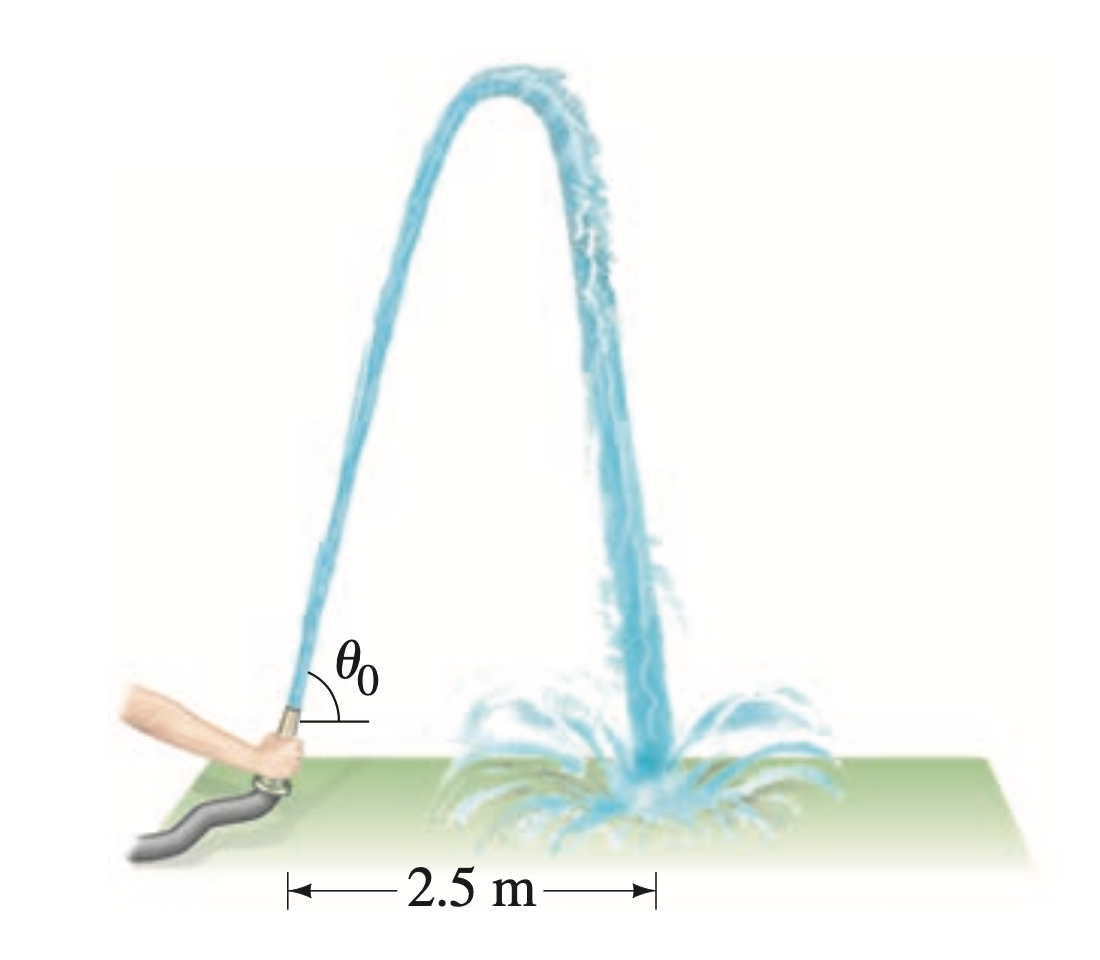
\includegraphics[width=2in]{images/slanga.png}
\end{wrapfigure}

\item Tígrisdýr stekkur lárétt fram af $\SI{7.5}{m}$ háum kletti með lárétta hraðanum $\SI{3.0}{m/s}$. Hversu langt frá kletsbrúninni mun tígrisdýrið lenda?


\item Bergljótu er fleygt lárétt út um gluggann á G-stofu með hraðanum $\SI{5.1}{m/s}$. Hversu langt frá Gamla skóla lendir hún ef glugginn er í $\SI{7.3}{m}$ hæð yfir jörðu?

\item Kafari nokkur hleypur með hraðanum $\SI{2.5}{m/s}$ lárétt fram af klettsbrún og lendir í vatninu $\SI{3.0}{s}$ síðar. Hversu hár var kletturinn og í hversu mikilli láréttri fjarlægð frá kletsbrúninni lenti kafarinn í vatninu?

\item Bolta er kastað með láréttum upphafshraða $\SI{12.2}{m/s}$ fram af toppi byggingar og lendir í láréttri fjarlægð, $\SI{21.0}{m}$, frá byggingunni. Hversu há er byggingin?


\item Kalli litli heldur vatnsslöngu við jörðina. Vatnið skýst út úr slöngunni með hraðanum $\SI{6.5}{m/s}$. Undir hvaða horni, $\theta_0$, á Kalli að halla slöngunni þannig að vatnið lendi í láréttri fjarlægð $\SI{2.5}{m}$ frá henni?

\end{minipage}

\begin{minipage}{\linewidth}

\begin{wrapfigure}{r}{1.4in}

\vspace{-1.4cm}
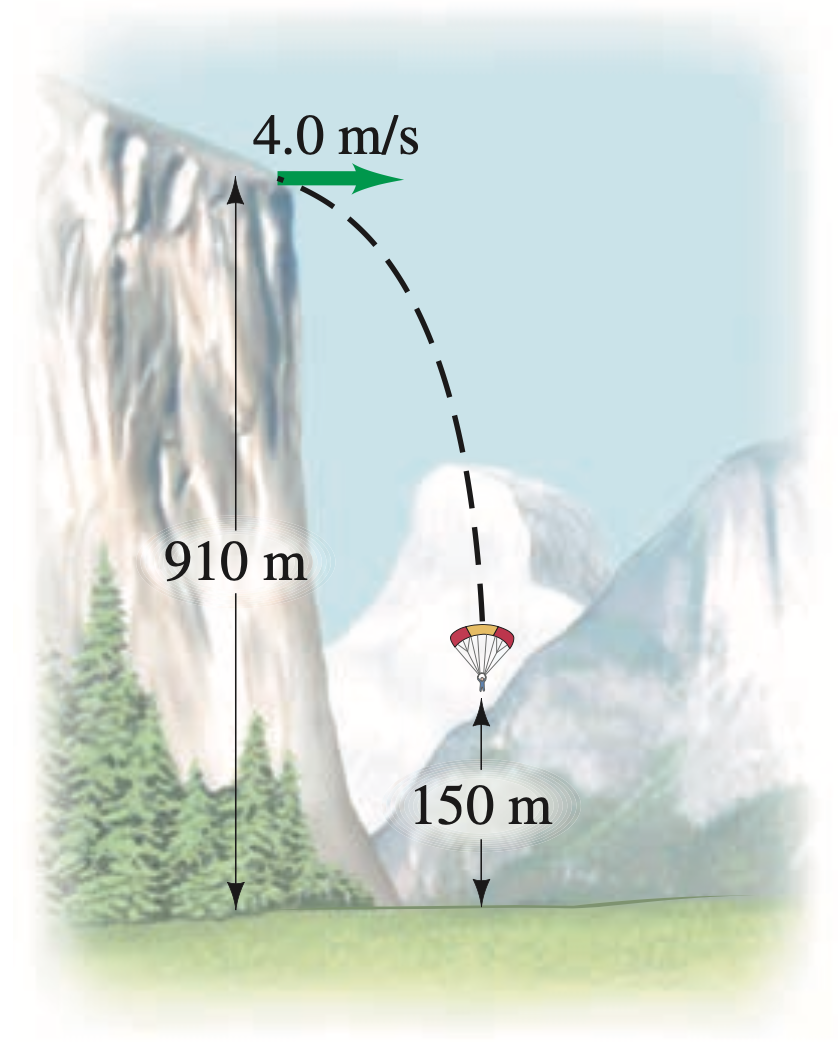
\includegraphics[width=2in]{images/hoppa.png}

\end{wrapfigure}

\item Ofurhugar eru þekktir fyrir að hoppa fram af El Capitan í Yosemite garðinum í Kaliforníu í Bandaríkjunum. Stokkið er úr $\SI{910}{m}$ hæð með láréttum upphafshraða $\SI{4.0}{m/s}$ fram af bjarginu. Til þess að lifa af fallið opna ofurhugarnir fallhlífar í $\SI{150}{m}$ hæð. Við hunsum loftmótstöðu í þessu dæmi.

\begin{enumerate}[label = \textbf{(\alph*)}]
    \item Hversu lengi eru ofurhugarnir í frjálsu falli áður en þeir opna fallhlífar sínar?
    \item Hversu langt frá fjallsbrúninni eru ofurhugarnir þegar þeir opna fallhlífar sínar?
\end{enumerate}

\item Ör er skotið af boga með upphafshraða $\SI{36.6}{m/s}$ undir horni $\theta = \ang{42.2}$ miðað við lárétt úr hæð $\SI{1.62}{m}$. Ákvarðið
\begin{enumerate}[label = \textbf{(\alph*)}]
    \item Mestu hæðina sem örin nær.
    \item Heildartíma örvarinnar í loftinu.
    \item Drægi örvarinnar, þ.e.a.s.~hvar hún lendir.
    \item Hraða örvarinnar $\SI{1.50}{s}$ eftir að henni var skotið af stað.
\end{enumerate}

\end{minipage}

\begin{minipage}{\linewidth}
\begin{wrapfigure}{r}{1.4in}
\vspace{-3.75cm}
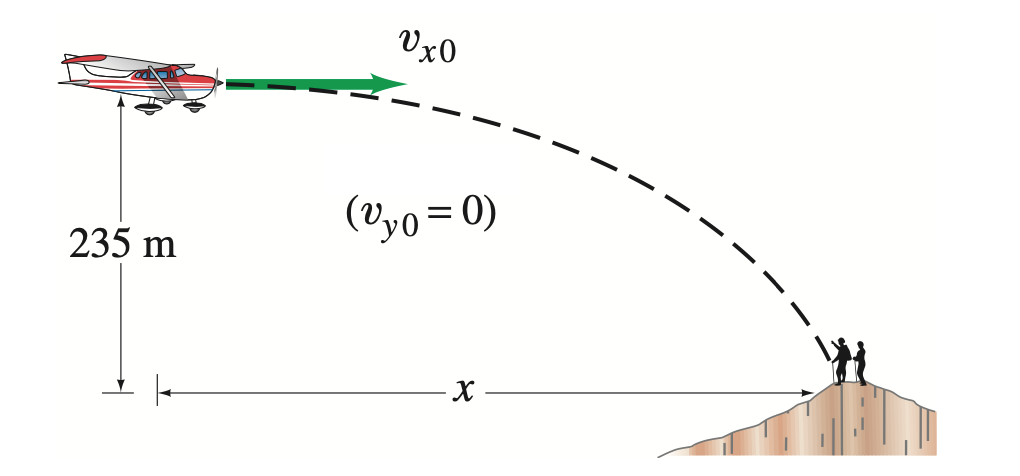
\includegraphics[width=2in]{images/flug.png}
\end{wrapfigure}

\item Björgunarflugvél ætlar að sleppa birgðum til fjallgöngumanna sem eru staddir á fjallstindi, $\SI{235}{m}$ fyrir neðan flughæð björgunarflugvélarinnar. Ef að flugvélin hefur láréttan hraða $\SI{69.4}{m/s}$ í hversu mikilli láréttri fjarlægð ætti flugvélin að sleppa birgðunum þannig að fjallgöngumennirnir geti gripið birgðirnar?

\end{minipage}

\vspace{1cm}

\begin{minipage}{\linewidth}
\vspace{-1cm}
\begin{wrapfigure}{r}{1.4in}
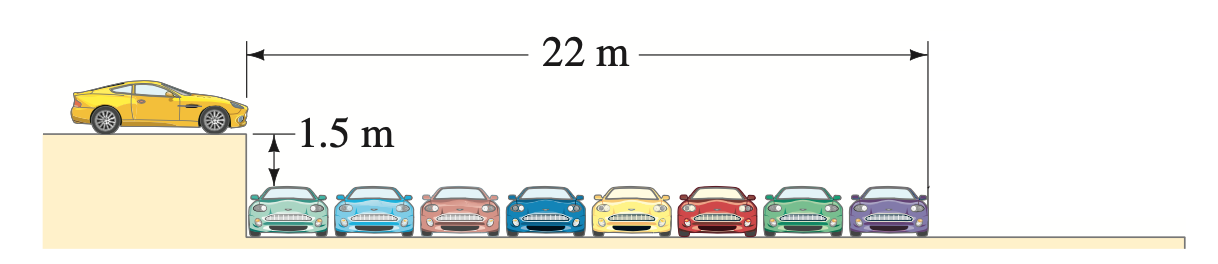
\includegraphics[width=2in]{images/bilalest.png}
\end{wrapfigure}

\item Glæfraökumaður ætlar að láta bílinn sinn stökkva yfir bílalest með $8$ bílum.
\begin{enumerate}[label = \textbf{(\alph*)}]
    \item Hver er minnsti hraðinn sem að hann þarf að keyra fram af láréttum stökkpallinum ef að lóðrétta fjarlægðin milli pallsins og bílanna er $\SI{1.50}{m}$ og lárétta vegalengdin sem hann þarf að komast er $\SI{22}{m}$?
    \item Ef að pallinum er núna hallað upp um horn $\theta = \ang{7.0}$ miðað við lárétt, hver er þá nýji lágmarkshraðinn sem hann þarf að stökkva fram af með?
\end{enumerate}

\end{minipage}

\item Slökkviliðsmaður skýtur vatni úr háþrýstislöngu í átt að brennandi byggingu. Hraði vatnsins við enda slöngunnar er \SI{25,0}{m/s}. Slökkviliðsmaðurinn stillir hornið $\theta = \SI{23}{\degree}$ sem slangan myndar við jörðu þannig að vatnið er \SI{3.00}{s} að ferðast til byggingarinnar. Gerum ráð fyrir því að slönguendinn nemi við jörðu.
\begin{enumerate}[label = \textbf{(\alph*)}]
    \item Hversu langt frá byggingunni stendur slökkviliðsmaðurinn?
\item Í hvaða hæð hæfir vatnið húsið?
\end{enumerate}

\newpage


\begin{minipage}{\linewidth}
\begin{wrapfigure}{r}{1.4in}
\vspace{-0.5cm}
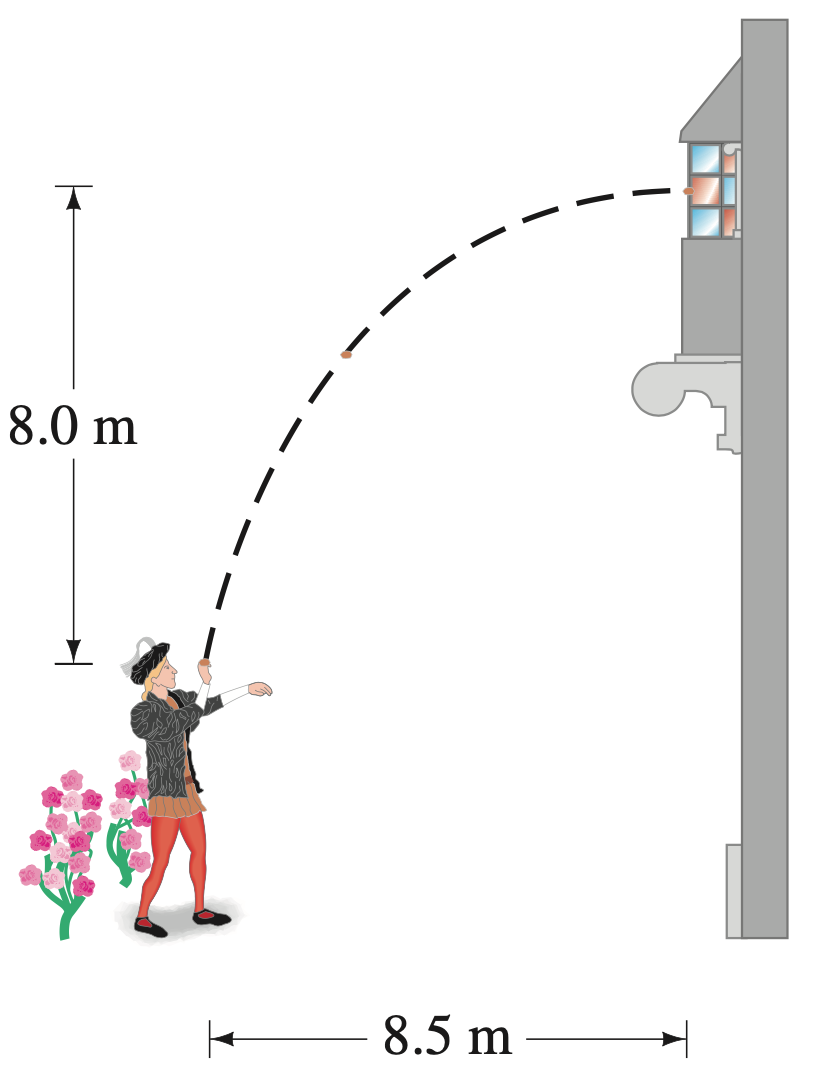
\includegraphics[width=2in]{images/romeo.png}
\end{wrapfigure}

\item Á Ólympíuleikum fatlaðra er keppt í Boccia. Markmið leiksins er að henda eigin bolta (rauður eða blár) sem næst hvítum bolta á afmörkuðum velli. Konráð Ragnarsson, Íslandsmeistari í Boccia, stendur $\SI{6.3}{m}$ frá hvítu kúlunni og kastar kúlunni sinni í átt að hvítu kúlunni úr $\SI{1.5}{m}$ hæð með hraðanum $\SI{7.0}{m/s}$ og horninu $\theta = \SI{47}{\degree}$ miðað við lárétt. Hversu langt frá hvítu kúlunni lendir kúla Konráðs?

\item Rómeó er að kasta steinum í gluggann hjá Júlíu. Hann kastar steinunum þannig að þeir lenda á glugganum aðeins með láréttan hraðaþátt. Hann stendur í rósagarðinum, $\SI{8.0}{m}$ fyrir neðan glugga Júlíu og í $\SI{8.5}{m}$ láréttri fjarlægð frá glugganum. Hver er hraði steinanna þegar þeir hæfa gluggann hennar Júlíu?

\item Tennisspilari slær boltann með hraðanum $v = \SI{15}{m/s}$ undir horninu $\theta = \SI{50}{\degree}$ miðað við lárétt. Þegar hann slær boltann er mótspilari hans í $d = \SI{10.0}{m}$ fjarlægð frá boltanum. Mótspilarinn byrjar að hlaupa $\SI{0.30}{s}$ eftir að boltinn er sleginn í von um að ná boltanum þegar hann er í $h = \SI{1.70}{m}$ hæð yfir upphafshæð.
\begin{enumerate}[label = \textbf{(\alph*)}]
    \item Hversu langur tími líður frá því að boltinn er sleginn þar til hann er í $\SI{1.70}{m}$ hæð á niðurleið?
    \item Á hvaða meðalhraða þarf mótspilarinn að hlaupa til þess að ná boltanum?
\end{enumerate}

\end{minipage}


\begin{minipage}{\linewidth}
\begin{wrapfigure}{r}{1.4in}
\vspace{-1.5cm}
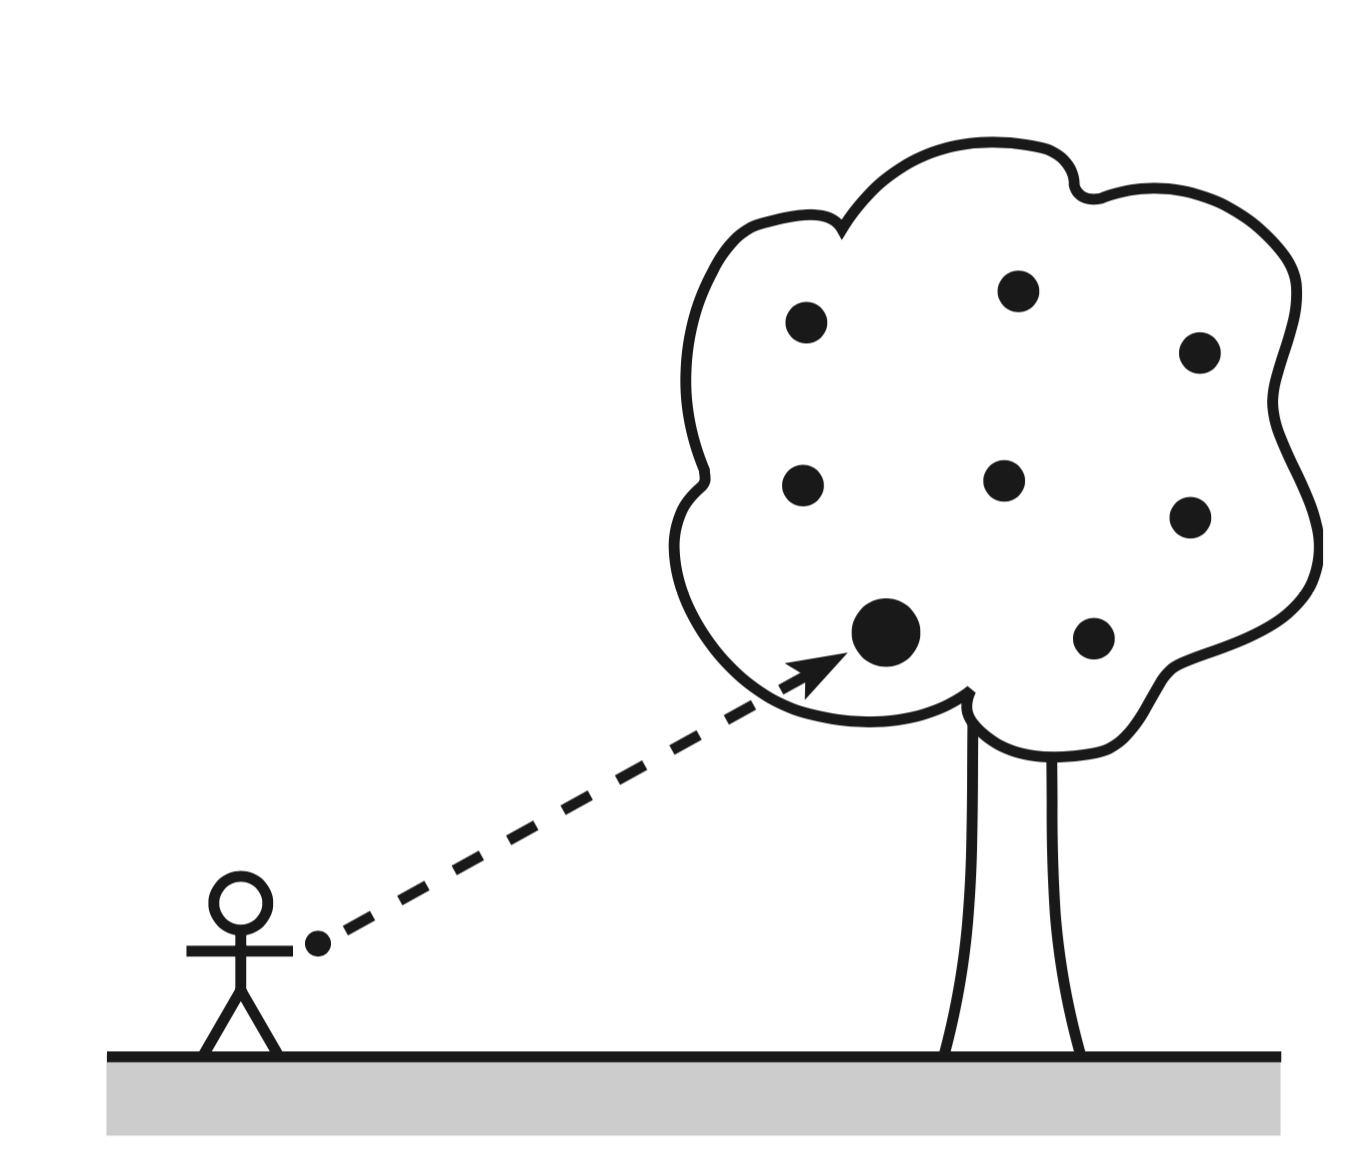
\includegraphics[width=2in]{images/epli.png}
\end{wrapfigure}

\item \textbf{(Jólapróf 2018)} Herbert heiðarlega langar í epli í hádegismat svo hann kastar stein í eplið. Hann stendur í láréttri fjarlægð, $\SI{5,4}{m}$, frá eplinu. Hann kastar steininum úr hæðinni $\SI{1,3}{m}$ með upphafshraða $\SI{13,1}{m/s}$  yfir horninu $\theta = \SI{37}{\degree}$ miðað við lárétt og hittir eplið.

\begin{enumerate}[label = \textbf{(\alph*)}]
\item Hversu langur tími leið frá því að Herbert kastaði steininum og þar til hann lenti á eplinu?
\item Í hvaða hæð var eplið?
\end{enumerate}

\end{minipage}

\item Hlut er kastað frá jörðu úr $(x_0, y_0) = (0,0)$ með upphafshraða $v_0$ yfir horninu $\theta$ miðað við lárétt. Sýnið:
\begin{enumerate}[label = \textbf{(\alph*)}]
    \item Tíminn sem líður frá því að boltanum er kastað og þar til hann er í mestri hæð er gefinn með:
    \begin{align*}
        t_{1/2} = \frac{v_0 \sin\theta}{g}.
    \end{align*}
    \item Heildartíminn sem líður frá því að boltanum er kastað og þar til hann lendir er gefinn með:
    \begin{align*}
        T = 2t_{1/2} = \frac{2v_0 \sin\theta}{g}.
    \end{align*}
    
    \item Mesta hæðin sem boltinn nær er gefin með:
    \begin{align*}
        y = \frac{{v_0}^2 \sin^2\theta}{2g}.
    \end{align*}
    
    \item Drægni boltans (lárétta færslan) er gefin með:
    \begin{align*}
        x = \frac{{v_0}^2 \sin(2\theta)}{g}.
    \end{align*}
    
    \item Notið niðurstöðuna úr liðum (c) og (d) til þess að finna yfir hvaða horni maður á að kasta til þess að boltinn nái mestri hæð og yfir hvaða horni maður á að kasta svo að boltinn komist sem lengst.
\end{enumerate}

\end{enumerate}

\newpage
